\documentclass[10pt,oneside]{article}

\usepackage{amsfonts}
\usepackage{amsmath}
\DeclareMathOperator*{\amax}{arg\,max}
\DeclareMathOperator*{\amin}{arg\,min}
\usepackage{amssymb}
\usepackage{dsfont}
\usepackage{bm}

\usepackage{epsf}
\usepackage{epsfig}
\usepackage{graphicx}
\usepackage{wrapfig} \usepackage{subfig}

\usepackage{enumerate}
\usepackage{listings}

\usepackage{setspace}
\usepackage{geometry}
\usepackage{fancyhdr}
%\usepackage{soul} % cross out text

\usepackage[latin2]{inputenc}
% \usepackage{times} % ez kiszedi a t1enc raszteressgt, de valami ms betu"tpust
% hasznl
\usepackage{lmodern} % ez eltu"nteti a raszteressget s mg jk is a betu"k
% \usepackage[magyar]{babel}
\usepackage{t1enc}

% \usepackage[T1]{fontenc}

\usepackage[usenames]{color}
\usepackage[colorlinks]{hyperref} 
\hypersetup{linkcolor=blue}
% \usepackage{showkeys}

% \onehalfspacing
\usepackage{indentfirst}
% \frenchspacing

\geometry{left=2.5cm,right=2.5cm,top=3.0cm,bottom=2.5cm}

\pagestyle{fancy}
\lhead{mufit2 model}
\chead{ }
\rhead{\thepage}

\lfoot{ }
\cfoot{ }
\rfoot{P\'{e}ter K\'{o}m\'{a}r, \the\year}


\renewcommand{\headrulewidth}{0.4pt}
\renewcommand{\footrulewidth}{0.0pt}

\newcommand{\refeq}[1]{Eq.(\ref{#1})}


% \numberwithin{equation}{section} \numberwithin{figure}{section}
% \numberwithin{table}{section}

\author{Peter Komar}
\title{mufit2 model}
\date{\today}




\begin{document}
\newcommand{\bel}{\begin{equation}}
\newcommand{\eel}{\end{equation}}
\newcommand{\be}{\begin{equation*}}
\newcommand{\ee}{\end{equation*}}

\newcommand{\bal}{\begin{eqnarray}}
\newcommand{\eal}{\end{eqnarray}}
\newcommand{\ba}{\begin{eqnarray*}}
\newcommand{\ea}{\end{eqnarray*}}

\newcommand{\ket}[1]{| #1 \rangle}
\newcommand{\Ket}[1]{\left| #1 \right\rangle}
\newcommand{\bra}[1]{\langle #1 |}
\newcommand{\Bra}[1]{\left\langle #1 \right|}

\newcommand{\no}{\noindent}

\newcommand{\ev}[1]{\langle #1 \rangle}
\newcommand{\Ev}[1]{\left\langle #1 \right\rangle}
\newcommand{\Tr}{\text{Tr}\,}
\newcommand{\T}{^\top}
\newcommand{\+}{^\dagger}
\newcommand{\s}{^\ast}
\newcommand{\PP}{\mathcal{P}}
\newcommand{\eqE}{= \!\!\!\!\!^{{}^{E}}\,}

\renewcommand{\d}[1]{\!d #1 \;}

\newcommand{\bE}{{\mathbf E}}
\newcommand{\bB}{{\mathbf B}}
\newcommand{\bF}{{\mathbf F}}
\newcommand{\bJ}{{\mathbf J}}
\newcommand{\bv}{{\mathbf v}}
\newcommand{\eps}{\varepsilon}
\newcommand{\br}{\mathbf r}
\newcommand{\bk}{\mathbf k}
\newcommand{\hatx}{\hat{\mathbf{x}}}
\newcommand{\haty}{\hat{\mathbf{y}}}
\newcommand{\hatz}{\hat{\mathbf{z}}}

\newcommand\independent{\protect\mathpalette{\protect\independenT}{\perp}}
\def\independenT#1#2{\mathrel{\rlap{$#1#2$}\mkern2mu{#1#2}}}


\renewcommand{\vec}[1]{{\bf #1}}
\newcommand{\mat}[1]{{\bf #1}}

\newcommand{\op}[1]{\mathbf{#1}}
\newcommand{\twovector}[2]{
	\left[
		\begin{array}{c}
		#1 \\
		#2
		\end{array}
	\right]
}
\newcommand{\threevector}[3]{
	\left[
		\begin{array}{c}
		#1 \\
		#2 \\
		#3
		\end{array}
	\right]
}
\newcommand{\fourvector}[4]{
	\left[
		\begin{array}{c}
		#1 \\
		#2 \\
		#3 \\
		#4
		\end{array}
	\right]
}
\newcommand{\fivevector}[5]{
	\left[
		\begin{array}{c}
		#1 \\
		#2 \\
		#3 \\
		#4 \\
		#5
		\end{array}
	\right]
}
\newcommand{\nvector}[2]{
	\left[
		\begin{array}{c}
		#1_1 \\
		#1_2 \\
		\vdots \\
		#1_#2
		\end{array}
	\right]
}
\newcommand{\ncovector}[2]{
	[#1_1\s, #1_2\s, \dots #1_#2\s]
}
\newcommand{\twobytwomatrix}[4]{
	\left[
		\begin{array}{cc}
		#1 & #2\\
		#3 & #4
		\end{array}
	\right]
}
\newcommand{\threebythreematrix}[9]{
	\left[
		\begin{array}{ccc}
		#1 & #2 & #3\\
		#4 & #5 & #6\\
		#7 & #8 & #9
		\end{array}
	\right]
}
\newcommand{\threebythreedeterminant}[9]{
	\left|
		\begin{array}{ccc}
		#1 & #2 & #3\\
		#4 & #5 & #6\\
		#7 & #8 & #9
		\end{array}
	\right|
}
\newcommand{\nbymmatrix}[3]{
	\left[ 
		\begin{array}{cccc}
		#1_{11}  & #1_{12} & \dots  & #1_{1 #2}\\
		#1_{21}  & #1_{22} &        &         \\
		\vdots   &         & \ddots & \vdots  \\
		#1_{#3 1}&         & \dots  & #1_{#3 #2}
		\end{array}
	\right]
}
\newcommand{\nbyndeterminant}[2]{
	\left|
		\begin{array}{cccc}
		#1_{11}  & #1_{12} & \dots  & #1_{1 #2}\\
		#1_{21}  & #1_{22} &        &         \\
		\vdots   &         & \ddots & \vdots  \\
		#1_{#2 1}&         & \dots  & #1_{#2 #2}
		\end{array}
	\right|
}


\newcommand{\argmax}[1]{\underset{#1}{\operatorname{arg}\operatorname{max}}\;}

\thispagestyle{empty}
\maketitle

We introduce a 2-level model, ``hidden Gaussian process'', for smoothening the inferred growth rate curves of optical density time series produced by a turbidostat.

 
%\newpage
\tableofcontents
\newpage

\lstset{
numbers=left, 
numberstyle=\small, 
numbersep=8pt, 
frame = single, 
language=Python, 
framexleftmargin=15pt
}


\section{Data}

\subsection{Raw optical density data}
We start with the time series of the raw optical density (OD) measurements recorded during a single experimental run of a turbidostat. At consecutive (but not necessarily equidistant) time points, OD is recorded. This produces two vectors of real numbers:
\begin{itemize}
	\item the time points, $\{\text{tp}_n\;:\; n = 1,2, \ldots N_\text{total}\}$, and
	\item the OD values, $\{\text{od}_n\;:\; n = 1,2, \ldots N_\text{total}\}$.
\end{itemize}
Under normal operating conditions, the time series (tp, od) has the following features:
\begin{itemize}
	\item a long initial growth from a low OD value to the operating OD regime,
	\item sharp drops of OD, when it reaches a predefined threshold value,
	\item gradual growth of OD between sharps drops, and
	\item intermittent spikes of OD.
\end{itemize}

\subsection{Preprocessing}
Out of the four features of the raw (tp, od) time series, we wish to model only the gradual growth (and maybe the initial growth) phases. For this we filter the time series and partition it into non-overlapping regions by 
\begin{enumerate}
	\item Using heuristic filters to identify sudden changes of od, and remove the associated data points.
	\item Group uninterrupted series of data points into non-overlapping regions.
	\item Take the logarithm of OD.
\end{enumerate}
This produces the cleaned time series $(t, x)$ of $N$ data points:
\ba
	t &=& (t_1, t_2, \ldots t_N), \quad \text{where}\; t_n \in \mathds{R},\quad \text{and}\; t_n < t_{n+1}, \\
	x &=& (x_1, x_2, \ldots x_N), \quad \text{where}\; x_n = \log(\text{od}) \in \mathds{R},
\ea
and a list of $R$ regions, i.e. non-overlapping sets $\mathcal{R}_r$,
\be
	r \in \{1, 2, \ldots R\},\qquad \text{where each }\mathcal{R}_r = \{s(r), s(r) + 1, \ldots e(r) - 1, e(r)\} \subset \{1, 2,\ldots N\}
\ee
is a list of consecutive indexes, where $s(r)$ is the first and $e(r)$ is the last.

\section{Model}

We model all $R$ regions of the cleaned time series $(t, x)$ with a single model that captures the gradual growth within each region as well as two features of between-region change of the growth rate ($\mu$), sudden changes and long-term drifts.

\subsection{Parameters}
We use the following unknown variables to describe the time series. The role of each value will become more clear in the next subsection.
\begin{itemize}
	\item $x_0 = \{x_{r,0}\;:\;r=1,2,\ldots R\} \in \mathds{R}^R$ represents the starting log-OD value at the beginning of each region.
	\item $\mu_1 = \{\mu_{r,1}\;:\;r=1,2,\ldots R\} \in \mathds{R}^R$  represents the growth rate at the beginning of each region.
	\item $\mu_2 = \{\mu_{r,2}\;:\;r=1,2,\ldots R\} \in \mathds{R}^R$  represents the growth rate at the end of each region.
	\item $\sigma_x \in \mathds{R}$ is the strength of measurement noise of log-OD.
	\item $\mu_0$ is $\mu$ at the beginning of the experiment.
	\item $\nu_0$ is the \emph{rate of change} of $\mu$ at the beginning of the experiment
	\item $D$ is the diffusion coefficient of the velocity of the long term drift of $\mu$.
	\item $\tau$ is the time scale of the short-term fluctuations of $\mu$.
	\item $\sigma_y$ is the magnitude of the short-term fluctuations of $\mu$.
\end{itemize}


\subsection{Individual regions}
We assume that for given $x_0, \mu_1, \mu_2$ values, the log-OD values in different regions become independent. This allows us to write the generating distribution of log-OD as 
\be
	P(x\;|\;t, x_0, \mu_1, \mu_2) = \prod_{r=1}^R P(x^{(r)}\;|\;t^{(r)}, x_{r,0}, \mu_{r,1}, \mu_{r,2})\quad ,
\ee
where $x^{(r)}$ and $t^{(r)}$ are the set of log-OD and time points belonging to region $r$.

Furthermore, within each region $r$, we assume that $\mu$ changes deterministically and linearly between $\mu_{r,1}$ (at $t_{s(r)}$) and $\mu_{r,2}$ (at $t_{e(r)}$), i.e.
\be
	\mu(t) = 
	\mu_{r,1} \frac{t_{e(r)} - t}{t_{e(r)} - t_{s(r)}} + 
	\mu_{r,2} \frac{t - t_{s(r)}}{t_{e(r)} - t_{s(r)}}\quad,\quad\text{if}\quad t_{s(r)} \leq t \leq t_{e(r)}\quad.
\ee
This leads to a quadratic time dependence for the ``noiseless'' log-OD,
\ba
	x_r^\text{noiseless}(t) 
	&=& 
	x_{r,0} + \intop_{t_{s(r)}}^{t} \d{t'} \mu(t') = 
	x_{r,0} + f_r(t)\,\mu_{r,1} + g_r(t)\,\mu_{r,2}\quad ,\text{ where }
	\\
	f_r(t) &=& \frac{t_{e(r)}(t - t_{s(r)}) - \frac{1}{2} (t^2 - t_{s(r)}^2)}{t_{e(r)} - t_{s(r)}}
	\\
	g_r(t) &=& \frac{\frac{1}{2}(t^2 - t_{s(r)}^2) - t_{s(r)}(t - t_{s(r)})}{t_{e(r)} - t_{s(r)}}
\ea
The noiseless log-OD deterministic (given $x_0, \mu_1, \mu_2$). If  we further assume that the measurement noise is uncorrelated between different time points, then each $x_n$ becomes independent from every other $x_{n'}$. Assuming Gaussian noise with strength $\sigma_x$, we can write their generating distribution as
\be
	P(x^{(r)}\;|\;t^{(r)}, x_{r,0}, \mu_{r,1}, \mu_{r,2}) = \prod_{n=s(r)}^{e(r)} \text{Normal}\Big(x_n\;\Big|\;\text{mean}=x_r^\text{noiseless}(t_n), \;\text{variance}=\sigma_x^2\Big)
\ee







\section{Type II maximum likelihood solution}

We wish to obtain robust estimates of $\mu$, and its statistical uncertainty. To do this, we follow the ``type II'' maximum likelihood procedure:
\begin{enumerate}
	\item We determine the maximum likelihood estimates of the parameters $\mu_0, \nu_0, D, \sigma_\mu, \tau$ and $\sigma_x$. (For this, we need a computationally efficient access to the marginal likelihood $P(x\;|\; \mu_0, \nu_0, D, \sigma_\mu, \tau, \sigma_x)$.)

	\item Using the MLE parameter values, we calculate the mean and standard deviation of each element of $\mu$.
\end{enumerate}

In this section, we derive a formula for the logarithm of the marginal likelihood, which can directly be implemented using matlab, python's numpy or stan.

\subsection{Expanding \refeq{eq:P_region}}
To better understand how data from each region $x^{(r)}$ determines the region-specific parameters $z_r = (x_{r,0}, \mu_{r,1}, \mu_{r,2})$, we expand \refeq{eq:P_region}.
\be
	P(x^{(r)}\;|\;z_r, \sigma_x) = \prod_{n=s(r)}^{e(r)} \text{Normal}\Big(x_n\;\Big|\; \text{mean} = x_{r,0} + f_r(t_n) \mu_{r,1} + g_r(t_n)\mu_{r,2},\; \text{variance} = \sigma_x^2\Big)
\ee
Now, we can expand the pdf of the normal distribution and write
\be
	P(x^{(r)}\;|\;z_r, \sigma_x) = \exp\left(-\frac{N_r}{2}\log(2\pi \sigma_x^2)\right) \;\exp\left(-\frac{1}{2\sigma_x^2} \sum_{n=s(r)}^{e(r)} \Big[x_{r,0} + f_r(t_n)\mu_{r,1} + g_r(t_n)\mu_{r,2} - x_n \Big]^2\right)
\ee
where $N_r = e(r) - s(r) + 1$. We expand the square bracket and distribute the summation on the terms. The result is a quadratic form of the vector $z_r$,
\ba
	-\frac{1}{2}\sum_{n=s(r)}^{e(r)}\Big[\ldots\Big]^2 &=& \gamma_r + b_r\T z_r - \frac{1}{2}z_r\T A_r z_r,\qquad \text{where}
	\\
	\gamma_r &=& -\frac{1}{2} \sum_{n=s(r)}^{e(r)} (x_n)^2
	\\
	b_r &=& \sum_{n=s(r)}^{e(r)}\threevector{x_n}{ x_nf_r(t_n) }{x_ng_r(t_n)}
	\\
	A_r &=& \sum_{n=s(r)}^{e(r)} \threebythreematrix
	{1}{ f_r(t_n)}{ g_r(t_n)}
	{ f_r(t_n)}{(f_r(t_n))^2}{f_r(t_n)g_r(t_n)}
	{ g_r(t_n)}{f_r(t_n)g_r(t_n)}{(g_r(t_n))^2}
\ea

When we consider all regions, their generating distribution can be written as 
\bal
	P(x\;|\;z,\sigma_x) &=& \prod_{r=1}^R P(x^{(r)}\;|\;z_r, \sigma_x)
	\nonumber\\
	&=& \exp\left(-\frac{N}{2}\log(2\pi \sigma_x^2)\right) \exp\left(\frac{1}{\sigma_x^2} \sum_{r=1}^R \Big[\gamma_r + b_r\T z_r - \frac{1}{2} z_r\T A_r z_r\Big]\right) \nonumber\\
\label{eq:Px|z}
	&=& \exp\left(-\frac{N}{2}\log(2\pi \sigma_x^2)\right) \exp\left(\frac{1}{\sigma_x^2} \Big[\gamma + b\T \tilde z - \frac{1}{2} \tilde z\T A \tilde z\Big]\right)
\eal
where the new variables $\gamma, b, A$ are (direct) sums of the individual $\gamma_r, b_r, A_r$ variables:
\be
	\gamma = \sum_{r=1}^R \gamma_r,\qquad b = \bigoplus_{r=1}^R b_r,\qquad A = \bigoplus_{r=1}^R A_r,
\ee 
where we define the direct sum of the matrices as the operation of concatenating them in a block-diagonal fashion. (Note: Since $\gamma, b, A$ do not depend on model parameters, we can compute them once and store their values to improve efficiency.)

\subsection{Expanding \refeq{eq:P_mu}}
Now, we expand the formula describing how the hyperparameters $\mu_0, \nu_0, D, \sigma_\mu, \tau$ affect the region-specific parameters $z_r = (x_{r,0}, \mu_{r,1}, \mu_{r,2})$. While \refeq{eq:P_mu} describes the joint distribution of all elements of $\mu_1$ and $\mu_2$, here we incorporate $x_0$ into the formula, and express the joint distribution of all elements of $z$ ($=S\tilde z$).
\bal
	\mu = \bigoplus_{r=1}^R (\mu_{r,1}, \mu_{r,2}) 
	&\sim& 
	\text{Multi-Normal}
	\Big(\mu\;\Big|\;
	\text{mean} = 
		\underbrace{
			m^\text{int.BM} + m^\text{sq.exp}
		}_{m^{(\mu)}},\,
	\text{cov} = 
		\underbrace{
			\Sigma^\text{int.BM} + \Sigma^\text{sq.exp}
		}_{\Sigma^{(\mu)}}
	\Big)
	\nonumber\\
	x_0 = \bigoplus_{r=1}^R x_{r,0} 
	& \sim &
	\text{Multi-Normal}
	\Big( x_0 \;\Big| \;
	\text{mean} = 
		\underbrace{
			\mathbf{1}_R \bar x
		}_{m^{(x_0)}},\,
	\text{cov} = 
		\underbrace{
			\mathbb{I}_{R\times R} \lambda^2(\Delta x)^2
		}_{\Sigma^{(x_0)}}
	\Big)
	\nonumber\\
	z = x_0\oplus \mu 
	&\sim &
	\text{Multi-Normal}\Big(z\;\Big|\;\text{mean} = m,\,\text{cov}=\Sigma\Big)\nonumber\\
\label{eq:Pz}
	&& 
	= 
	\exp\left(-\frac{1}{2}\log\Big(\det (2\pi \Sigma)\Big)\right)\,
	\exp\left(-\frac{1}{2}(z - m)\T \Sigma^{-1} (z-m)\right)
\eal
where $\mathbf{1}_R$ is the all-1 vector, and $\mathbb{I}_{R\times R}$ is the identity matrix, and the mean and covariance of $z$ can be written as 
\be
	m = m^{(x_0)} \oplus m^{(\mu)},\qquad
	\Sigma = \Sigma^{(x_0)} \oplus \Sigma^{(\mu)}
\ee
where the direct sum ($\oplus$) is defined as concatenation between vectors and block-diagonal composition between matrices. Separating the determinant and the inverse operations on the $x_0$ and the $\mu$ spaces,
\ba
	\Sigma^{-1} &=& \Big(\Sigma^{(x_0)}\Big)^{-1} \oplus \Big(\Sigma^{(\mu)}\Big)^{-1}\quad,\\
	\log\Big(\det(2\pi \Sigma)\Big) &=& 3R \log(2\pi) + \log\Big(\det(\Sigma^{(x_0)})\Big) + \log\Big(\det(\Sigma^{(\mu)})\Big)\quad,
\ea
will lead more efficient calculations because $m^{(x_0)}$ and $\Sigma^{(x_0)}$ are known but $m^{(\mu)}$ and $\Sigma^{(\mu)}$ are unknown, and need to be evaluated at every iteration step during fitting.

\subsection{Eliminating $z$}
Multiplying \refeq{eq:Pz} and \refeq{eq:Px|z}, and converting $\tilde z$ to $z$ using the definition of the permutation matrix $S$ from \refeq{eq:def_S} ($\tilde z = S\T z$) yields the likelihood in the following quadratic exponential form
\ba
	P(x\;|\;z) \,P(z) &=& 
	\exp\left(-\frac{N}{2}\log(2\pi \sigma_x^2)\right) 
	\exp\left(\frac{1}{\sigma_x^2} \Big[\gamma + (Sb)\T z - \frac{1}{2} z\T (S A S\T) z\Big]\right) \times \\
	&& 
	\exp\left(-\frac{1}{2}\log\Big(\det (2\pi \Sigma)\Big)\right)\,
	\exp\left(-\frac{1}{2}(z - m)\T \Sigma^{-1} (z-m)\right)
	\\
	&=& \exp\left(-\frac{1}{2}z\T\mathcal{A} z + \mathcal{B}\T z + \mathcal{C}\right)
\ea
where
\ba
	\mathcal{A} &=& \frac{1}{\sigma_x^2}SAS\T + \Sigma^{-1} \\
	\mathcal{B} &=& \frac{1}{\sigma_x^2} Sb + \Sigma^{-1}m \\
	\mathcal{C} &=& -\frac{N}{2}\log(2\pi \sigma_x^2) -\frac{1}{2}\log\Big(\det (2\pi \Sigma)\Big) + \frac{\gamma}{\sigma_x^2} - \frac{1}{2}m\T \Sigma^{-1}m\quad.
\ea

To eliminate $z$ from the likelihood, we integrate with respect to $z$. Using the result for such a Gaussian integral (see Appendix \ref{app:gaussian_integral}), we obtain
\be
	P(x) = \int\d{z} P(x\;|\;z)P(z) = \int\d{z} \exp\left(-\frac{1}{2}z\T\mathcal{A} z + \mathcal{B}\T z  + \mathcal{C}\right) = \sqrt{\frac{(2\pi)^{3R}}{\det(\mathcal{A})}} \exp\left(\frac{1}{2}\mathcal{B}\T\mathcal{A}^{-1}\mathcal{B} + \mathcal{C}\right)\quad.
\ee
Taking the logarithm yields the log likelihood as a function of the data $x$ and the hyperparameters $\mu_0$, $\nu_0$, $D$, $\sigma_\mu$, $\tau$, $\sigma_x$,
\bel
\label{eq:L}
	L\big(\mu_0, \nu_0, D, \sigma_\mu, \tau, \sigma_x\big) = \log P(x) = \frac{3R}{2}\log(2\pi) - \frac{1}{2}\log\Big(\det(\mathcal{A})\Big) + \frac{1}{2}\mathcal{B}\T\mathcal{A}^{-1}\mathcal{B} + \mathcal{C}\quad.
\eel

We can start from realistic values for the hyperparameters, use gradient-based optimization methods to find maximum of $L$. This yields the maximum likelihood estimates $\mu_0\s$, $\nu_0\s$, $D\s$, $\sigma_\mu\s$, $\tau\s$, $\sigma_x\s$.

\subsection{Posterior mean and variance of $\mu$}
We can use the maximum likelihood estimates of $\mu_0\s$, $\nu_0\s$, $D\s$, $\sigma_\mu\s$, $\tau\s$, $\sigma_x\s$ to calculate the mean and variance of the growth rate from the joint distribution
\be
	P(x, z) = P(x\;|\;z) P(z) = \exp\left(-\frac{1}{2}z\T \mathcal{A} z + \mathcal{B}\T z + \mathcal{C}\right)\quad,
\ee
which, after dividing it with $P(x)$ (which is just a normalization constant from the point of view of $z$) yields the conditional probability
\ba
	P(z\;|\;x) &=& \frac{P(x,z)}{P(x)} \propto \exp\left(-\frac{1}{2}z\T \mathcal{A} z + \mathcal{B}\T z \right) \propto \exp\left(-\frac{1}{2}\Big(z - \mathcal{A}^{-1}\mathcal{B}\Big)\T\mathcal{A}\Big(z - \mathcal{A}^{-1}\mathcal{B}\Big)\right)
	\\
	&=&
	\text{Multi-Normal}\Big(z\;\Big|\;\text{mean} = \mathcal{A}^{-1}\mathcal{B},\;\text{cov}=\mathcal{A}^{-1}\Big)\quad,
\ea
which means that each component of $z$ ($x_{r,0}$ and $\mu_{r,1}, \mu_{r,2}$) is distributed as a normal distribution. Remembering that $z = x_0 \oplus \mu$, we can express the mean and variance of each element of $\mu \in \mathds{R}^{2R}$ as
\bel
	\mathbb{E}(\mu_i\;|\;x, \mu_0\s, \nu_0\s, D\s, \sigma_\mu\s, \tau\s, \sigma_x\s) = \Big[\mathcal{A}^{-1}\mathcal{B}\Big]_{R+i}\quad,\qquad
	\text{var}(\mu_i\;|\;x, \mu_0\s, \nu_0\s, D\s, \sigma_\mu\s, \tau\s, \sigma_x\s) = \Big[\mathcal{A}^{-1}\Big]_{R+i,\,R+i}\quad.
\eel


\begin{appendix}
\section{Derivations}


\subsection{Mean and covariance of integral of Brownian motion}
\label{app:intBM}
Shifted Brownian motion is defined as a Gaussian process $\nu(t)$ on $t \geq 0$, with mean and covariance functions defined as
\be
	m^{(\nu)}(t) = \nu_0
	\quad,\qquad 
	K^{(\nu)}(t, t') = D\,\text{min}(t, t')\quad,
\ee
where $\nu_0$ is the starting point at $t = 0$, and $D$ is the diffusion coefficient of the Brownian motion.

We define the integral of the Brownian motion as the process $\mu(t) = \mu_0 + \intop_0^t \d{x} \nu(x)$ on $t \geq 0$, with mean and covariance functions defined as
\be
	m^{(\mu)}(t) = \mu_0 + \intop_0^{t} \d{x} m^{(\nu)}(x) = \mu_0 + \nu_0 t
	\quad,\qquad
	K^{(\mu)}(t, t') = \intop_0^t \d{x} \intop_0^{t'} \d{y} K^{(\nu)}(x, y)
\ee
The double integral can be separated into 3 non-overlapping parts. With the notation $l = \text{min}(t, t')$ and $h = \text{max}(t, t')$, we can write 
\be
	K^{(\mu)}(t, t') = D\intop_0^h \d{x} \intop_0^{l} \d{y} \text{min}(x, y)
\ee
since $K^{(\nu)}(x,y) = D\,\text{min}(x,y)$ is symmetric in its arguments. The integration domain can be partitioned into three non-overlapping domains,
\begin{figure}[h]
\centering
	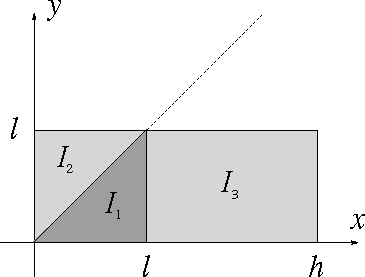
\includegraphics[width=0.3\textwidth]{figs/I1I2I3_regions.pdf}
\end{figure}
\ba
	I_1 &=& \intop_0^l \d{x} \intop_0^x \d{y} \underbrace{\text{min}(x,y)}_{y} \;=\; \intop_0^l \d{x} \frac{x^2}{2} \;=\; \frac{l^3}{6}
	\\
	I_2 &=& \intop_0^l \d{y} \intop_0^y \d{x} \underbrace{\text{min}(x,y)}_{x} \;=\; \intop_0^l \d{y} \frac{y^2}{2} \;=\; \frac{l^3}{6}
	\\
	I_3 &=& \intop_l^h \d{x} \intop_0^l \d{y} \underbrace{\text{min}(x,y)}_{y} \;=\; \intop_l^h \d{x} \frac{l^2}{2} \;=\; (h-l)\frac{l^2}{2}
\ea
the sum of which yields
\be
	K^{(\mu)}(t, t') = D(I_1 + I_2 + I_3) = D\,\frac{l^2}{2}\left(h - \frac{l}{3}\right)  = D\,\frac{\text{min}(t, t')^2}{2}\left(\text{max}(t, t') - \frac{\text{min}(t, t')}{3}\right)
\ee

\subsection{Gaussian integral}
\label{app:gaussian_integral}
Here we calculate the following multi-dimensional Gaussian integral, where $z, \mathcal{B} \in \mathds{R}^n$, $\mathcal{A}\in \mathds{R}^{n\times n}$ (positive definite) and $\mathcal{C} \in \mathds{R}$, 
\ba
	I &:=& \int\d{z} \exp\left(-\frac{1}{2}z\T \mathcal{A} z + \mathcal{B}\T z + \mathcal{C}\right) \\
	&= &
	\int\d{z} \exp\left(-\frac{1}{2}z\T \mathcal{A} z + \frac{1}{2}z\T \mathcal{B} + \frac{1}{2}\mathcal{B}\T z + \mathcal{C}\right) \\
	&=&
	\int\d{z} \exp\left(-\frac{1}{2}\Big(z - \mathcal{A}^{-1}\mathcal{B}\Big)\T \mathcal{A} \Big(z - \mathcal{A}^{-1}\mathcal{B}\Big) + \frac{1}{2}\mathcal{B}\T\mathcal{A}^{-1}\mathcal{B} + \mathcal{C}\right)\\
	&=&
	\exp\left(\frac{1}{2}\mathcal{B}\T\mathcal{A}^{-1}\mathcal{B} + \mathcal{C}\right) \int\d{z'} \exp\left(-\frac{1}{2}(z')\T \mathcal{A} z'\Big)\right).
\ea
Since $\mathcal{A}$ is positive definite there exists an orthogonal matrix $\mathcal{O}$ that diagonalizes it, 
\be
	\mathcal{OAO}\T = \Lambda = \text{diag}(\lambda_1, \lambda_2, \ldots \lambda_n)
\ee
where $\lambda_i$ are the eigenvalues of $\mathcal{A}$. In terms of the transformed coordinates $z'' = \mathcal{O}z'$ we get a separable integral:
\be
	\int\d{z'} \exp\left(-\frac{1}{2}(z')\T \mathcal{A} z'\Big)\right) = \int\d{z''} \exp\left(-\frac{1}{2}(z'')\T \Lambda z''\Big)\right) = \prod_{i=1}^n \int\d{x_i} \exp\left(-\frac{1}{2}x_i \lambda_i x_i\Big)\right)
\ee
Each factor can be simplified using the result for a 1-dimensional Gaussian integral $\int\d{x}\exp(-\frac{1}{2}ax^2) = \sqrt{2\pi / a}$, giving
\be
	\prod_{i=1}^n \sqrt{2\pi / \lambda_i} = \sqrt{\frac{(2\pi)^n}{\prod_i \lambda_i}} = \sqrt{\frac{(2\pi)^n}{\text{det}(\Lambda)}} = \sqrt{\frac{(2\pi)^n}{\text{det}(\mathcal{A})}},
\ee
where $\det{(\Lambda)} = \det{(\mathcal{A})}$, because the transformation matrix $\mathcal{O}$ is orthogonal, i.e. $\det\mathcal{(O)} = 1$. This results in
\be
	I = \exp\left(\frac{1}{2}\mathcal{B}\T\mathcal{A}^{-1}\mathcal{B} + \mathcal{C}\right)\times \sqrt{\frac{(2\pi)^n}{\text{det}(\mathcal{A})}}\quad.
\ee

\section{Implementation}

\subsection{Stan code for \refeq{eq:L}}

\end{appendix}


\end{document}